% Project 3 report. Compile with pdfLaTeX (on Overleaf: upload this whole folder, main document = main.tex).
% The tables in tables/ are written by src/make_tables.py from results/results_table.csv and results/analysis.json
% (params.tex and versions.tex by hand). Numbers in the text were copied from the same files.
\documentclass[11pt,a4paper]{article}
\usepackage[T1]{fontenc}
\usepackage[margin=2.3cm]{geometry}
\usepackage{graphicx}
\usepackage{booktabs}
\usepackage{amsmath}
\usepackage{xcolor}
\usepackage{placeins}
\usepackage[font=small,labelfont=bf]{caption}
\usepackage[colorlinks=true,linkcolor=blue!50!black,urlcolor=blue!50!black,citecolor=blue!50!black]{hyperref}

\setlength{\parindent}{0pt}
\setlength{\parskip}{0.55em}

\title{Anchor-Based Object Recognition and Localization\\[2pt]\large R7020E Computer Vision and Image Processing -- Project 3}
\author{Group 6: Achyuth Kumar Baddela, Sathish Kumaresan, Suresh Balaraman}
\date{28 October 2026}

\begin{document}
\maketitle

\begin{abstract}
Given three photos (anchors) of one specific fire extinguisher, the system decides for every frame of a robot video whether
that extinguisher is present and, if so, draws a box around it. Printed pictures of extinguishers placed around the room must
not be accepted. The system finds red candidate regions, scores each one against the anchors with a frozen DINOv2 embedding,
lowers the score of candidates that look like flat prints using the depth image, and accepts the best candidate if its score is
above a threshold chosen on a development sequence. On the held-out sequence it finds the extinguisher in all 126 frames with no
false accepts. Three methods (a colour-histogram baseline, SIFT, and DINOv2) are each run with and without the depth cues, and a seventh system with the cues but no matcher shows what the matcher adds. All code runs on a CPU.
\end{abstract}

%------------------------------------------------------------------------------------------------
\section{Task and data}
\textbf{Anchors.} Three full-resolution phone photos (3024$\times$4032 px) of the same CO$_2$ extinguisher from three viewpoints (Figure~\ref{fig:anchors}).
Each photo is cut down to the extinguisher with the same red-region rule that is used for the video frames.

\textbf{Frames.} Two recordings from a robot-mounted RGB-D camera: \texttt{test} and \texttt{eval}. Colour frames are 640$\times$400 px
with strong wide-angle distortion. The recordings also contain depth images, which arrive at a different rate; every colour frame is paired
with the depth frame nearest in time (Table~\ref{tab:counts}). The real extinguisher stands on the floor and the camera moves around it.
Printed pictures of extinguishers are fixed to block pillars around the room and act as decoys.

\begin{figure}[htbp]\centering
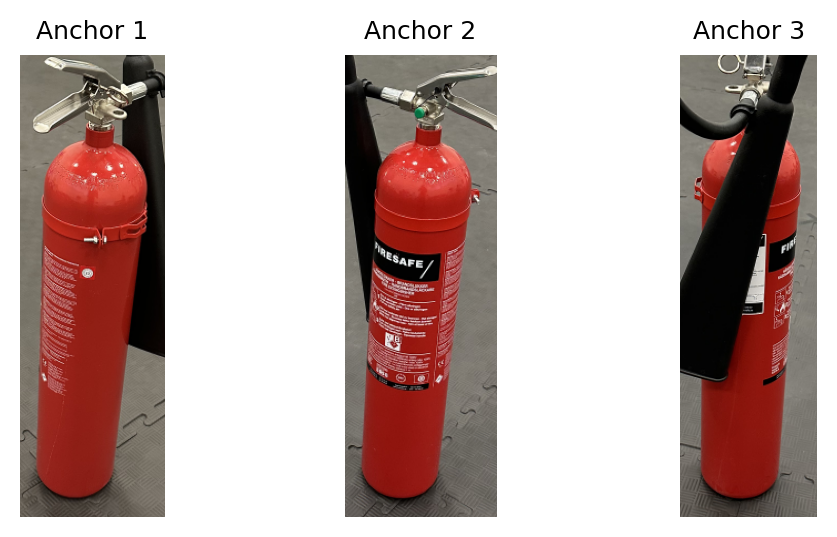
\includegraphics[width=0.55\linewidth]{figures/anchors.png}
\caption{The three anchors after cutting them down to the extinguisher.}\label{fig:anchors}
\end{figure}

\begin{table}[htbp]\centering\small
\begin{tabular}{llrrrrr}
\toprule
Sequence & Role & Frames & Present & Absent & Candidates & Depth gap (ms) \\
\midrule
\texttt{test} & development (tuned) & 93 & 54 & 39 & 150 & 28 / 95 \\
\texttt{eval} & held out & 126 & 126 & 0 & 350 & 29 / 65 \\
\bottomrule
\end{tabular}

\caption{The two sequences. ``Candidates'' is the number of red regions found by the candidate step.}\label{tab:counts}
\end{table}

%------------------------------------------------------------------------------------------------
\section{System architecture and design}
Figure~\ref{fig:arch} shows the system. No network is trained. The candidate regions and the depth cue features are shared; each of the three methods then runs in its own lane, with the cue penalty as an optional stage.

\begin{figure}[htbp]\centering
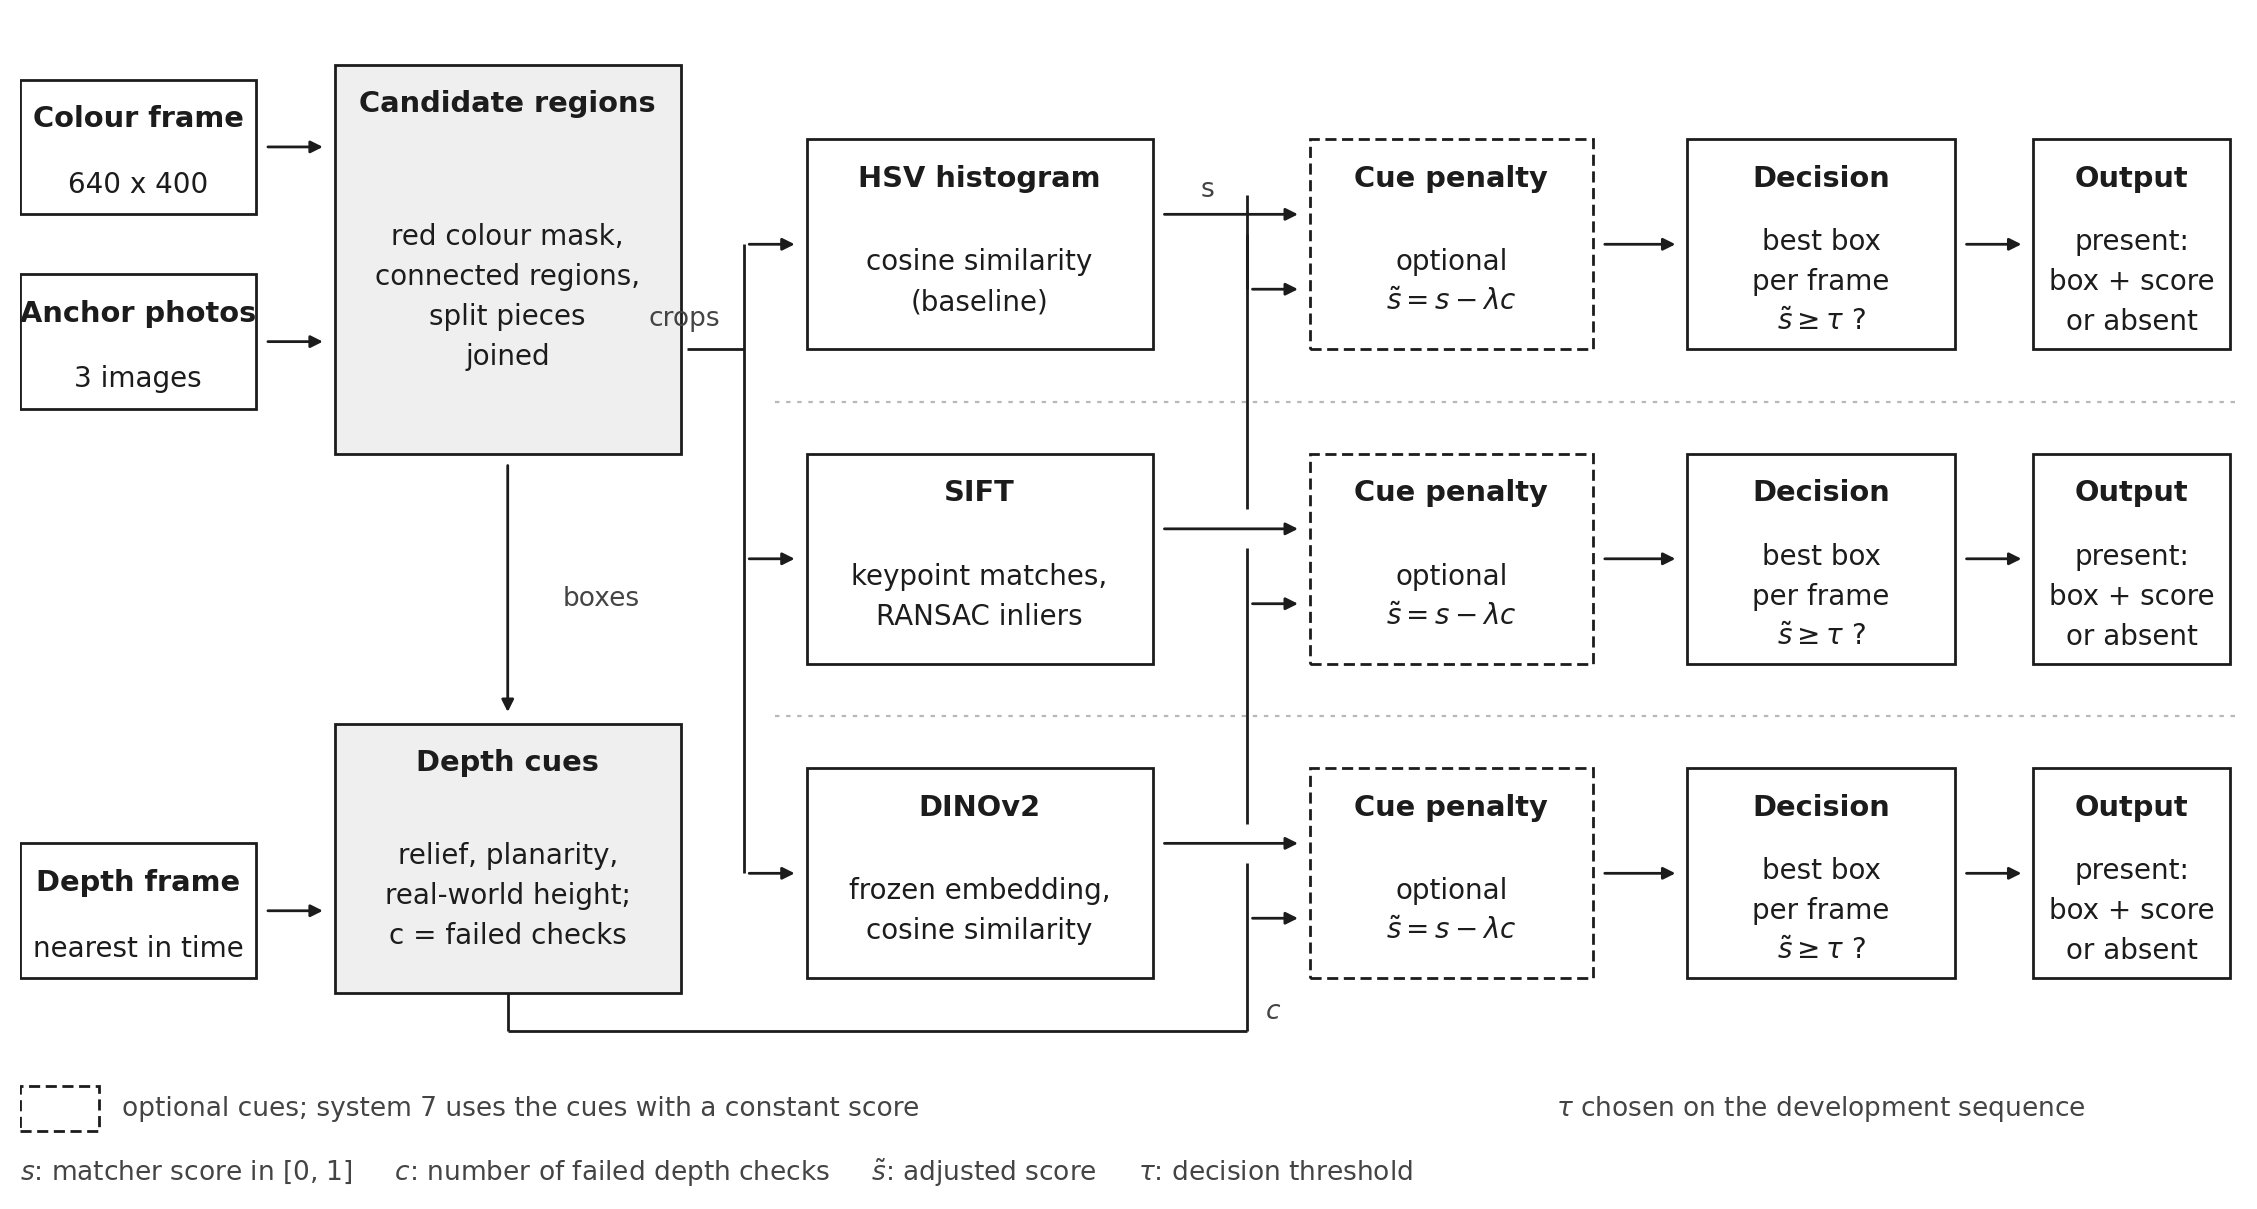
\includegraphics[width=\linewidth]{figures/architecture.png}
\caption{System architecture. One lane per method. The dashed stage gives six matcher variants, with and without cues; a seventh ablation uses cues and a constant score.}\label{fig:arch}
\end{figure}

\subsection{Candidate regions}
Both the real extinguisher and the printed pictures are red, so every tall red region becomes a candidate. Red pixels are found with OpenCV \cite{bradski2000} in HSV space
(hue near 0, high saturation), cleaned with a small morphological opening and closing, and grouped into connected regions. A region must be at least
40 px in area and taller than wide. The black hose crosses the red body and splits it in two, so red pieces directly above or below a region
(gap at most 20\% of the body height, not wider than 1.5 times the body) are joined to it. At most six candidates per frame are kept.
The width and gap constraints limit the inclusion of unrelated red objects. A candidate reaches at least 70\% overlap with the reference box in 179 of 180 target frames; the labels share the same red-region initialisation, as discussed in Section~3.

\subsection{Features and comparison with the anchors}
The crop of a candidate (box plus a margin that takes in the valve on top) is compared with the crops of the three anchors.
Two matchers are used, each producing one score in $[0,1]$.

\textbf{SIFT.} Keypoints and descriptors are computed on the anchor and the candidate, both resized to a height of 160 px. Descriptors are matched with
Lowe's ratio test (0.8) \cite{lowe2004}. RANSAC \cite{fischler1981} fits a rotation-scale-shift transform (a similarity: four degrees of freedom, so two correspondences fix it, which matters with only 3 to 10 good matches) and the number of inliers is counted.
The score is the best anchor's inlier count divided by 15, capped at 1; 15 is roughly the inlier count of a clear match at 160 px height, so the constant only sets the scale of the score and the threshold is tuned afterwards.

\textbf{DINOv2.} A frozen DINOv2 ViT-S/14 (21M parameters, pretrained by Meta without labels \cite{oquab2023}, run on the CPU, about 40 ms per crop) turns a crop into a
384-number embedding (the class token). The score is the cosine similarity to the anchor embeddings, rescaled from $[-1,1]$ to $[0,1]$.
Because the anchors are sharp phone photos and the video frames are small and blurry, each anchor is embedded at several resolutions
(shrunk to 40, 70, 112 and 200 px height and enlarged again); the best of all views counts. This is intended to reduce the resolution mismatch; its separate effect is not measured by a single-resolution ablation.

\subsection{Depth cues}
Both matchers only judge appearance, and a good print has the right appearance. The depth image gives physical evidence (Figure~\ref{fig:cues}).
For each candidate three numbers are computed from the depth pixels inside its box:
\begin{itemize}\setlength{\itemsep}{0pt}
\item \emph{Relief}: median depth of a ring around the box (30\% of the box width and height on every side, the box itself cut out) minus median depth inside it. A free-standing object has surroundings that are farther away; a print is part of its pillar.
\item \emph{Plane residual}: root-mean-square axial depth residual from the fitted surface $z=a u+b v+c$, where $u,v$ are pixel coordinates. This is an empirical flatness cue, not perpendicular distance to a calibrated 3D plane. A print is flat, the cylinder is not.
\item \emph{Real-world height}: pixel height $\times$ depth / focal length (306 px, from the camera calibration). The extinguisher is about 0.6 m tall; most printed pictures are smaller.
\end{itemize}
A candidate fails the \emph{flat} check if relief is below 100 mm and the plane residual is below 200 mm, and fails the \emph{size} check if its height is outside 0.45--1.0 m.
These limits were chosen on the development sequence only: the setting that lets the fewest print candidates through while keeping at least 95\% of the real extinguisher boxes. Stricter settings started rejecting real extinguishers whose depth was noisy at the edges, so the cues are allowed to lose one real box in twenty.
Candidates without a valid depth reading are not penalised.
The number of failed checks is multiplied by a penalty and subtracted from the matcher score. A hard rejection (veto) was also tried; the better of veto and penalties 0.05, 0.1, 0.2 is chosen per system on the development sequence.

\begin{figure}[htbp]\centering
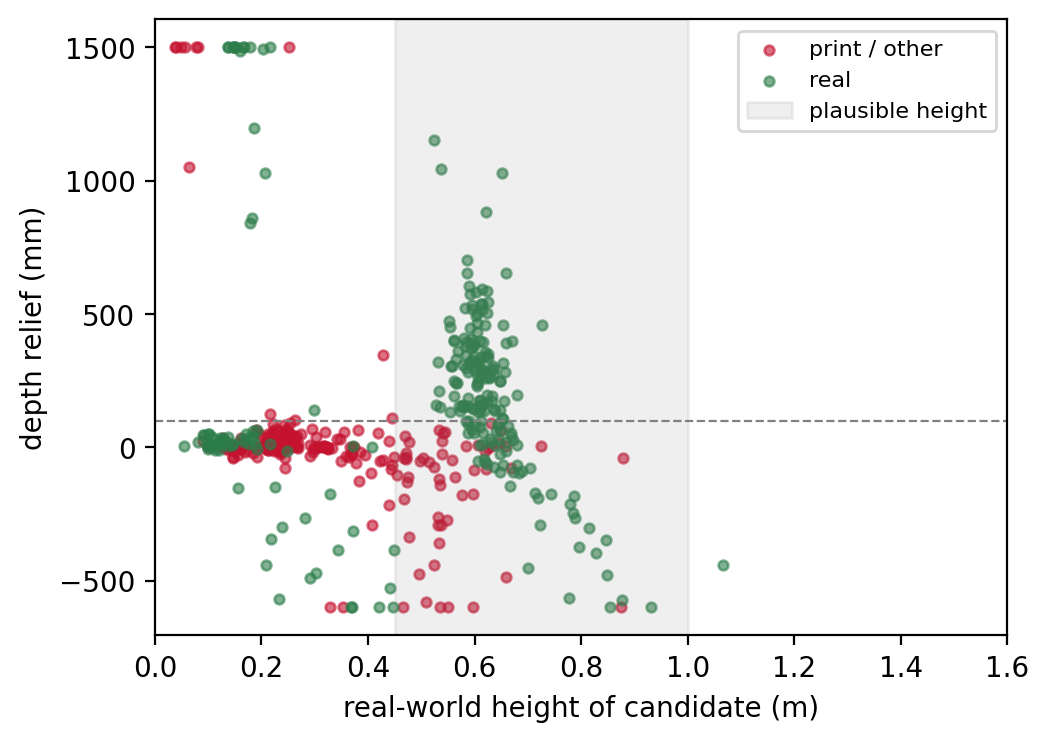
\includegraphics[width=0.62\linewidth]{figures/cue_separation.png}
\caption{Real-world height and depth relief of every candidate (both sequences). Green: the real extinguisher. Red: prints and other red regions. Grey band: plausible height.}\label{fig:cues}
\end{figure}

\subsection{Decision rule and output}
Every candidate is scored, so the candidates of a frame are ranked by their score (the full ranking is in \texttt{data/scores\_*.csv}). The candidate with the highest (penalised) score is the answer, because the target is a single object. If its score reaches the threshold $\tau$ the frame is \emph{target present} and the
candidate's box and score are output; otherwise \emph{target absent}. The threshold is the one with the highest recall on the development sequence among those with precision of at least 0.75
(if none reaches 0.75, the best F1). It is then fixed and applied unchanged to the held-out sequence.

\subsection{Baseline and compared systems}
The baseline is the course-suggested global colour histogram: a hue-saturation histogram of each candidate crop is compared with the anchors' histograms by cosine similarity.
Seven systems are compared, all on the same frames, candidates and thresholding rule: histogram baseline, SIFT and DINOv2, each without and with the depth cues, and a seventh system that keeps the candidates and the cues but has no matcher at all (every candidate scores 1, the biggest surviving red region is reported). The seventh system provides a candidate-and-cue reference; its effective acceptance rule is discussed in the results. DINOv2 + cues is the final system.
Because the baseline reuses the red candidates, it is a stronger baseline than a histogram over arbitrary windows would be.

%------------------------------------------------------------------------------------------------
\FloatBarrier
\section{Evaluation setup}
\textbf{Sequences.} \texttt{test} (93 frames: 54 with the target, 39 with only prints visible) is the development sequence; all thresholds and cue settings are tuned there.
\texttt{eval} (126 frames, all with the target) is held-out and used for the reported results. The folder names are those of the provided data. We did not split each sequence in two instead, because consecutive frames are near-duplicates and a within-sequence split would leak from tuning into evaluation.

\textbf{Reference boxes and labels.} The data contains no labels, so we labelled every frame ourselves in a small browser tool (\texttt{src/label\_tool.py}).
The tool shows an automatic red-region guess that is accepted or corrected by hand. Each frame is marked present or absent, and present frames get a box around the red body of the real extinguisher (hose excluded);
printed pictures are never the target. Boxes were checked and corrected where needed; 112 of the 126 \texttt{eval} boxes and 56 of the 93 \texttt{test} labels kept the automatic guess, which is the same red-region rule that produces the candidates. Localization success therefore measures whether the right region was chosen, not how tightly the box fits.

\textbf{Correctness rule.} A localization is correct if the centre of the predicted box lies inside the reference box.
\emph{TP}: target present and a correctly placed box accepted. \emph{FP}: any accepted box that is not a TP, i.e.\ a print, another object, or a wrongly placed box on a present frame.
\emph{FN}: target present but not correctly detected. Hence a wrongly placed accepted box counts as both an FP and an FN.
\[\text{precision}=\frac{TP}{TP+FP},\qquad \text{recall}=\frac{TP}{\#\text{frames with target}},\]
\[\text{localization success}=\frac{TP}{\#\text{all accepted detections}}.\]
An accepted print, other object or misplaced box fails localization, including on target-absent frames. With one output box per frame, localization success equals precision under this correctness rule; the tables also report correct/accepted counts.

\textbf{Thresholds and parameters.} Table~\ref{tab:thr} lists the decision threshold of each system and Table~\ref{tab:params} the other settings.
Table~\ref{tab:versions} gives the software versions.

\begin{table}[htbp]\centering\small
\begin{tabular}{lrl}
\toprule
System & Decision threshold $\tau$ & Cue handling \\
\midrule
HSV histogram (baseline) & 0.33 & -- \\
HSV + cues & 0.33 & penalty 0.05 \\
SIFT & 0.00 & -- \\
SIFT + cues & 0.00 & veto \\
DINOv2 & 0.78 & -- \\
DINOv2 + cues (final) & 0.76 & penalty 0.05 \\
candidates + cues, no matcher & 1.00 & penalty 0.05 \\
\bottomrule
\end{tabular}

\caption{Decision threshold and cue handling of each system, chosen on \texttt{test}. The SIFT threshold is 0: without cues no threshold reaches a precision of 0.75, so the rule falls back to the best F1, which lies at 0; with cues a precision of 0.95 is already reached at 0, so the highest-recall rule stops there. The SIFT score threshold therefore rejects no surviving candidate. Frames with no candidates, or with all candidates vetoed by cues, are still rejected. For system 7 every candidate scores 1 and a threshold of 1 with penalty 0.05 is the same as a veto.}\label{tab:thr}
\end{table}

\begin{table}[htbp]\centering\small
\begin{tabular}{lp{10.5cm}}
\toprule
Part & Setting \\
\midrule
Candidate step & red hue $[0,10]\cup[170,180]$, saturation $\ge 120$, value $\ge 70$; minimum area 40 px; height $\ge 1.2\times$ width; at most 6 candidates \\
Joining hose-split pieces & gap $\le 0.2\times$ body height, width $\le 1.5\times$ body width \\
Crop around a box & $+15\%$ sides, $+20\%$ top, $+5\%$ bottom \\
SIFT & contrast threshold 0.02; crops resized to height 160 px; ratio test 0.8; RANSAC similarity transform, 4 px; score = inliers / 15, capped at 1 \\
DINOv2 & dinov2\_vits14, frozen; CLS token of a $112\times56$ px crop; anchors also embedded at heights 40, 70, 112, 200 px; score = (max cosine + 1) / 2 \\
Depth cues & relief $\ge 100$ mm or plane RMS $\ge 200$ mm; height 0.45--1.0 m; focal length 306.1 px \\
Depth pairing & nearest depth frame in time, at most 100 ms apart \\
Threshold rule & highest recall on \texttt{test} with precision $\ge 0.75$ \\
Cue penalty options & 0.05, 0.1, 0.2 per failed check, or reject (veto); chosen on dev \\
\bottomrule
\end{tabular}

\caption{Main parameters (all in \texttt{configs/default.yaml} or at the top of the module that uses them).}\label{tab:params}
\end{table}

\begin{table}[htbp]\centering\small
\begin{tabular}{ll}
\toprule
Software & Version \\
\midrule
Python & 3.14.2 \\
OpenCV & 4.13.0 \\
NumPy & 2.4.2 \\
pandas & 3.0.0 \\
Matplotlib & 3.10.8 \\
PyTorch (CPU) & 2.10.0+cpu \\
torchvision & 0.25.0+cpu \\
DINOv2 weights & facebookresearch/dinov2, dinov2\_vits14 \\
\bottomrule
\end{tabular}

\caption{Software used. Everything ran on a CPU; no GPU is needed.}\label{tab:versions}
\end{table}

%------------------------------------------------------------------------------------------------
\FloatBarrier
\section{Results}
Table~\ref{tab:res_eval} shows the held-out sequence and Table~\ref{tab:res_test} the development sequence, on which the thresholds were tuned.
The course targets are precision $\ge$ 75\% and recall $\ge$ 60\%.

\begin{table}[htbp]\centering\small
\begin{tabular}{lrrrrrrr}
\toprule
System & Precision & Recall & TP & FP & FN & Loc.\ success & ms/frame \\
\midrule
HSV histogram (baseline) & 1.00 & 0.98 & 124 & 0 & 2 & 100\% (124/124) & 4 \\
HSV + cues & 1.00 & 0.96 & 121 & 0 & 5 & 100\% (121/121) & 4 \\
SIFT & 0.66 & 0.66 & 83 & 43 & 43 & 66\% (83/126) & 19 \\
SIFT + cues & 0.97 & 0.93 & 117 & 3 & 9 & 98\% (117/120) & 19 \\
DINOv2 & 1.00 & 0.99 & 125 & 0 & 1 & 100\% (125/125) & 114 \\
DINOv2 + cues (final) & 1.00 & 1.00 & 126 & 0 & 0 & 100\% (126/126) & 114 \\
candidates + cues, no matcher & 1.00 & 0.95 & 120 & 0 & 6 & 100\% (120/120) & 4 \\
\bottomrule
\end{tabular}

\caption{Held-out sequence \texttt{eval} (126 frames, all with the target). Loc.\ success = TP / all accepted detections, with correct/accepted counts in brackets. ms/frame: CPU time for candidates and matcher; DINOv2 takes longer here than on \texttt{test} because \texttt{eval} has 2.8 candidates per frame against 1.7.}\label{tab:res_eval}
\end{table}

\begin{table}[htbp]\centering\small
\begin{tabular}{lrrrrrrr}
\toprule
System & Precision & Recall & TP & FP & FN & Loc.\ success & ms/frame \\
\midrule
HSV histogram (baseline) & 0.84 & 1.00 & 54 & 10 & 0 & 84\% (54/64) & 5 \\
HSV + cues & 0.92 & 1.00 & 54 & 5 & 0 & 92\% (54/59) & 5 \\
SIFT & 0.49 & 0.83 & 45 & 46 & 9 & 49\% (45/91) & 18 \\
SIFT + cues & 0.95 & 0.96 & 52 & 3 & 2 & 95\% (52/55) & 18 \\
DINOv2 & 0.88 & 0.96 & 52 & 7 & 2 & 88\% (52/59) & 123 \\
DINOv2 + cues (final) & 0.95 & 1.00 & 54 & 3 & 0 & 95\% (54/57) & 123 \\
candidates + cues, no matcher & 0.95 & 0.96 & 52 & 3 & 2 & 95\% (52/55) & 5 \\
\bottomrule
\end{tabular}

\caption{Development sequence \texttt{test} (93 frames: 54 with the target, 39 with only prints). Thresholds were tuned on this sequence, so these numbers are optimistic.}\label{tab:res_test}
\end{table}

\textbf{What the numbers say.}
\begin{itemize}\setlength{\itemsep}{0pt}
\item The final system (DINOv2 + cues) finds the extinguisher in all 126 \texttt{eval} frames with no false accepts, and in all 54 target frames of \texttt{test}, with 3 false accepts, all on frames that show only prints.
\item SIFT alone cannot separate the real extinguisher from the prints: on \texttt{test} it accepts almost every frame, and on \texttt{eval} it often picks the wrong region (precision and recall 0.66).
\item The seventh system, candidates and cues with no matcher, scores 0.95 / 0.96 on \texttt{test}, the same as SIFT + cues, and 1.00 / 0.95 on \texttt{eval}. DINOv2 with a soft cue penalty recovers two target frames on \texttt{test} and six on \texttt{eval} that the no-matcher system rejects after one failed depth check. In all eight, the no-matcher system selects a correct region before rejecting it. The comparison therefore combines appearance evidence with a different effective acceptance rule; it does not isolate box ranking alone.
\item The depth cues help every matcher. On \texttt{test}, SIFT's precision rises from 0.49 to 0.95, DINOv2's from 0.88 to 0.95, and the histogram's from 0.84 to 0.92.
\item The histogram baseline is strong on \texttt{eval} (precision 1.00, recall 0.98), because every frame contains the target and the largest red region is usually the real extinguisher. It is clearly weaker on \texttt{test}, where it accepts 10 frames with only prints (precision 0.84).
\item \textbf{Limitation of the held-out sequence.} \texttt{eval} contains no frames without the target, so it cannot show whether a system rejects prints when the real object is absent. That is measured only on \texttt{test}, which is also the tuning sequence. The held-out result therefore says more about localization than about decoy rejection.
\end{itemize}

\begin{figure}[htbp]\centering
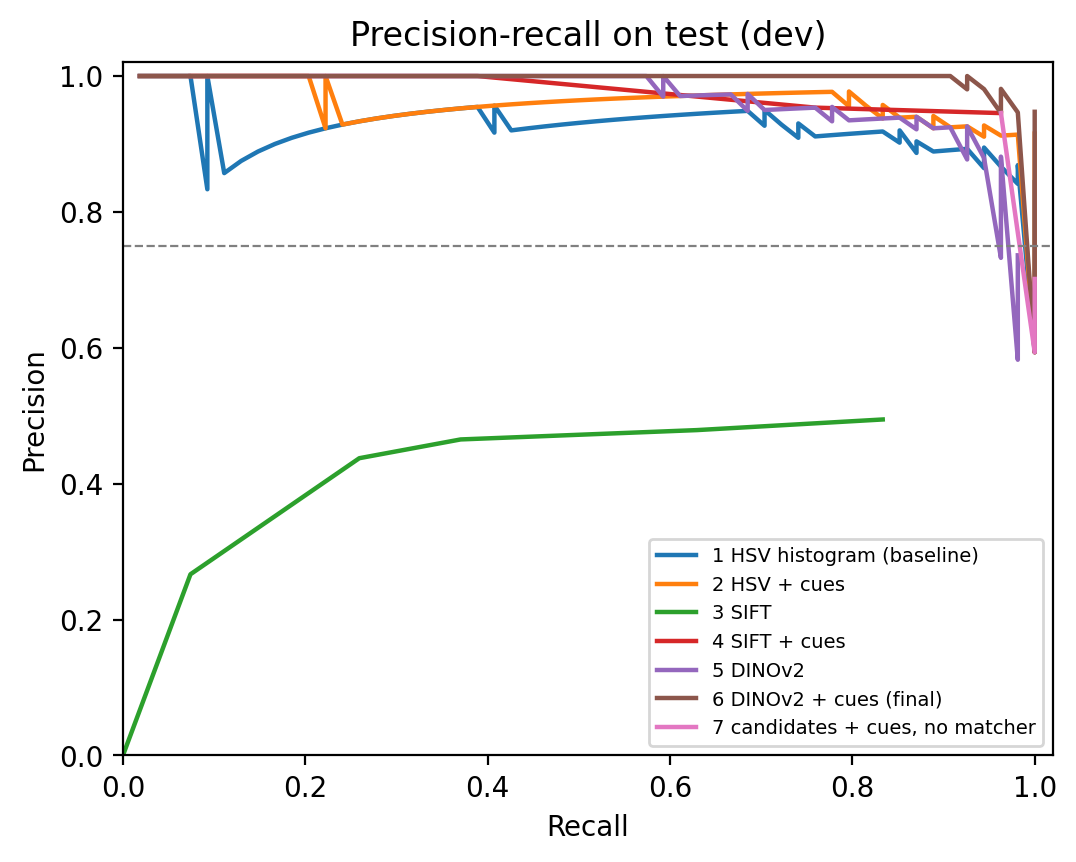
\includegraphics[width=0.62\linewidth]{figures/pr_curves_dev.png}
\caption{Precision-recall curves of the compared systems on \texttt{test}. The dashed line is the required precision of 0.75.}\label{fig:pr}
\end{figure}

%------------------------------------------------------------------------------------------------
\FloatBarrier
\section{Visual evidence}
Figure~\ref{fig:examples} shows the four cases the task asks for. In this run the final system has no missed target in either sequence, so that panel is empty.
Figure~\ref{fig:sift} shows SIFT matches for a real candidate and for a print, and Figure~\ref{fig:scores} the score distributions that explain the results.
Figure~\ref{fig:time} follows the final system's score through each sequence.

\begin{figure}[htbp]\centering
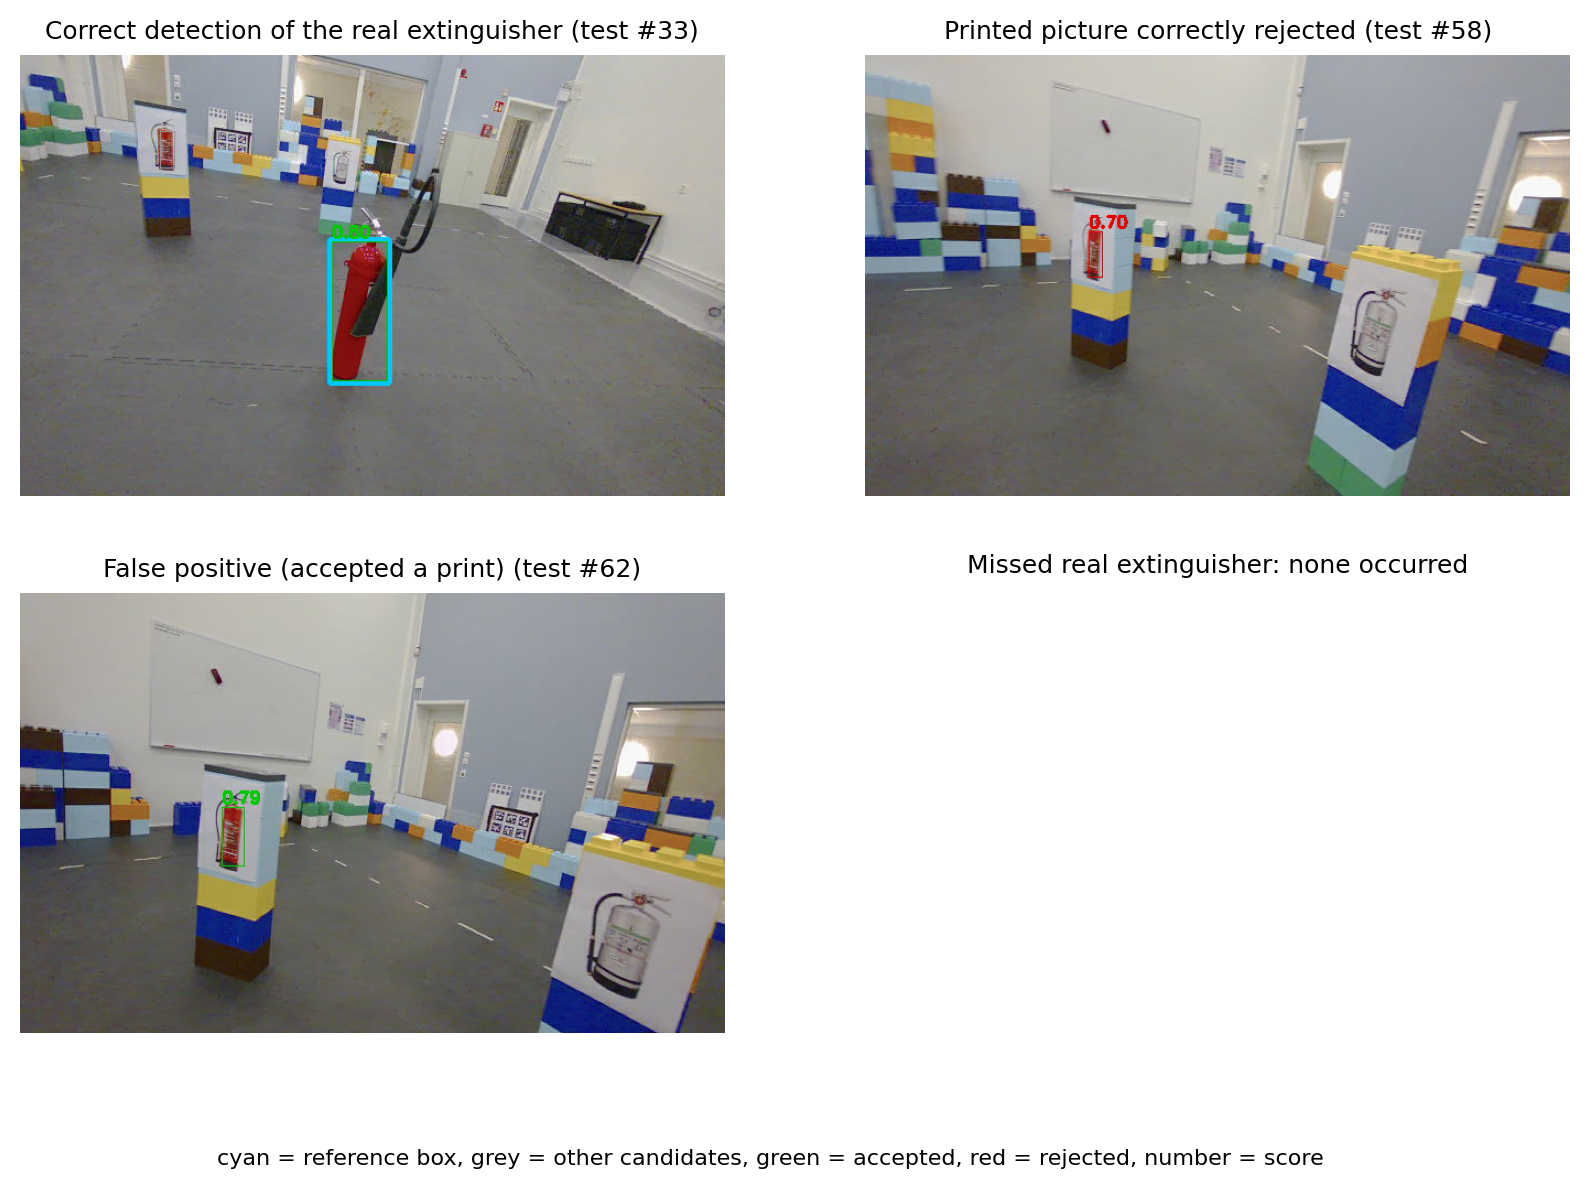
\includegraphics[width=\linewidth]{figures/examples.png}
\caption{Examples from the final system. Top left: correct detection. Top right: a printed picture that is correctly rejected. Bottom left: a print that is wrongly accepted. Bottom right: a missed target, if one occurred.}\label{fig:examples}
\end{figure}

\begin{figure}[htbp]\centering
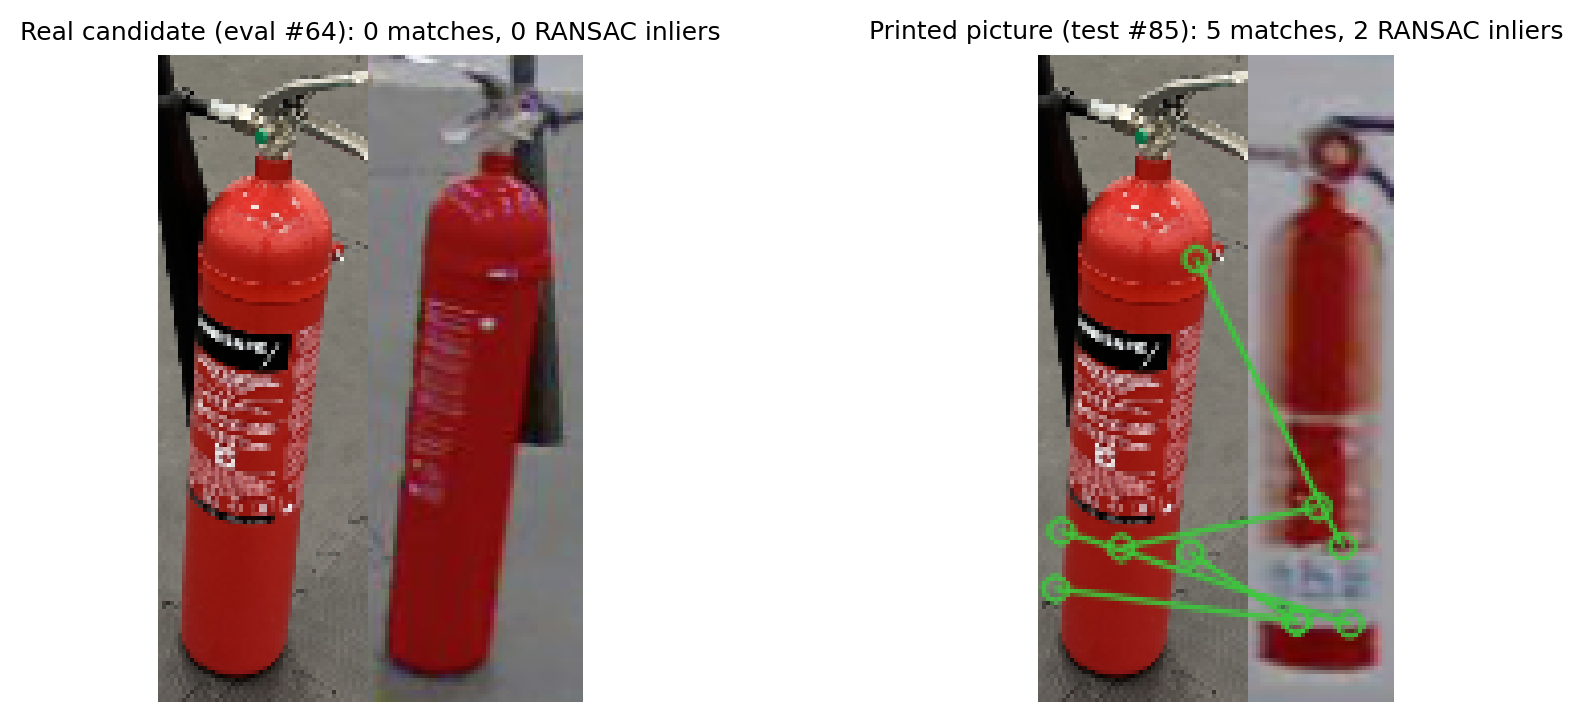
\includegraphics[width=0.9\linewidth]{figures/sift_matches.png}
\caption{SIFT correspondences (green lines) between anchor 2 and a real candidate (left) and a print (right). Few or no consistent matches are found for either.}\label{fig:sift}
\end{figure}

\begin{figure}[htbp]\centering
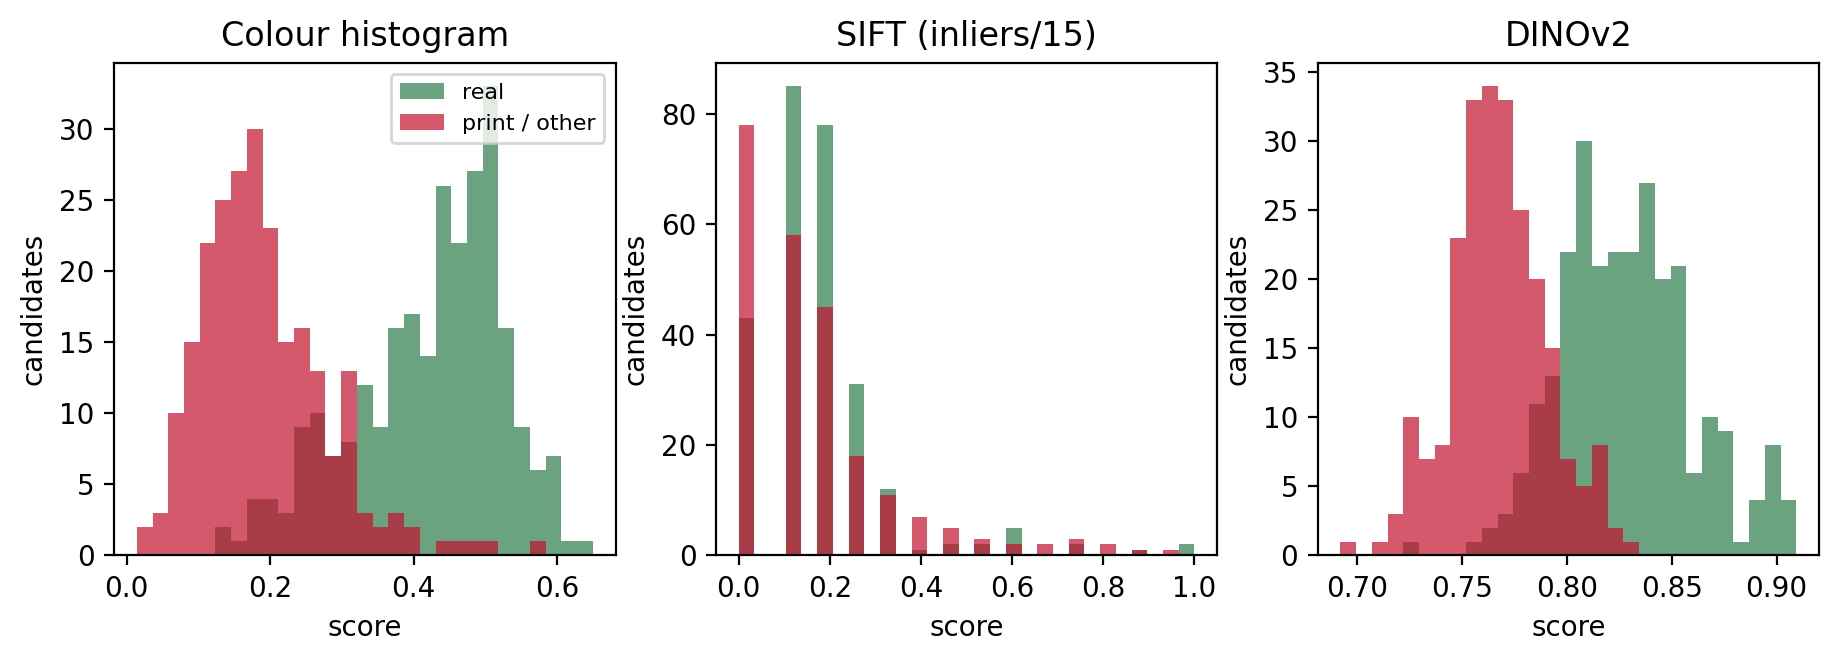
\includegraphics[width=\linewidth]{figures/score_distributions.png}
\caption{Score of real candidates and of print / other candidates for each matcher (both sequences).}\label{fig:scores}
\end{figure}

\begin{figure}[htbp]\centering
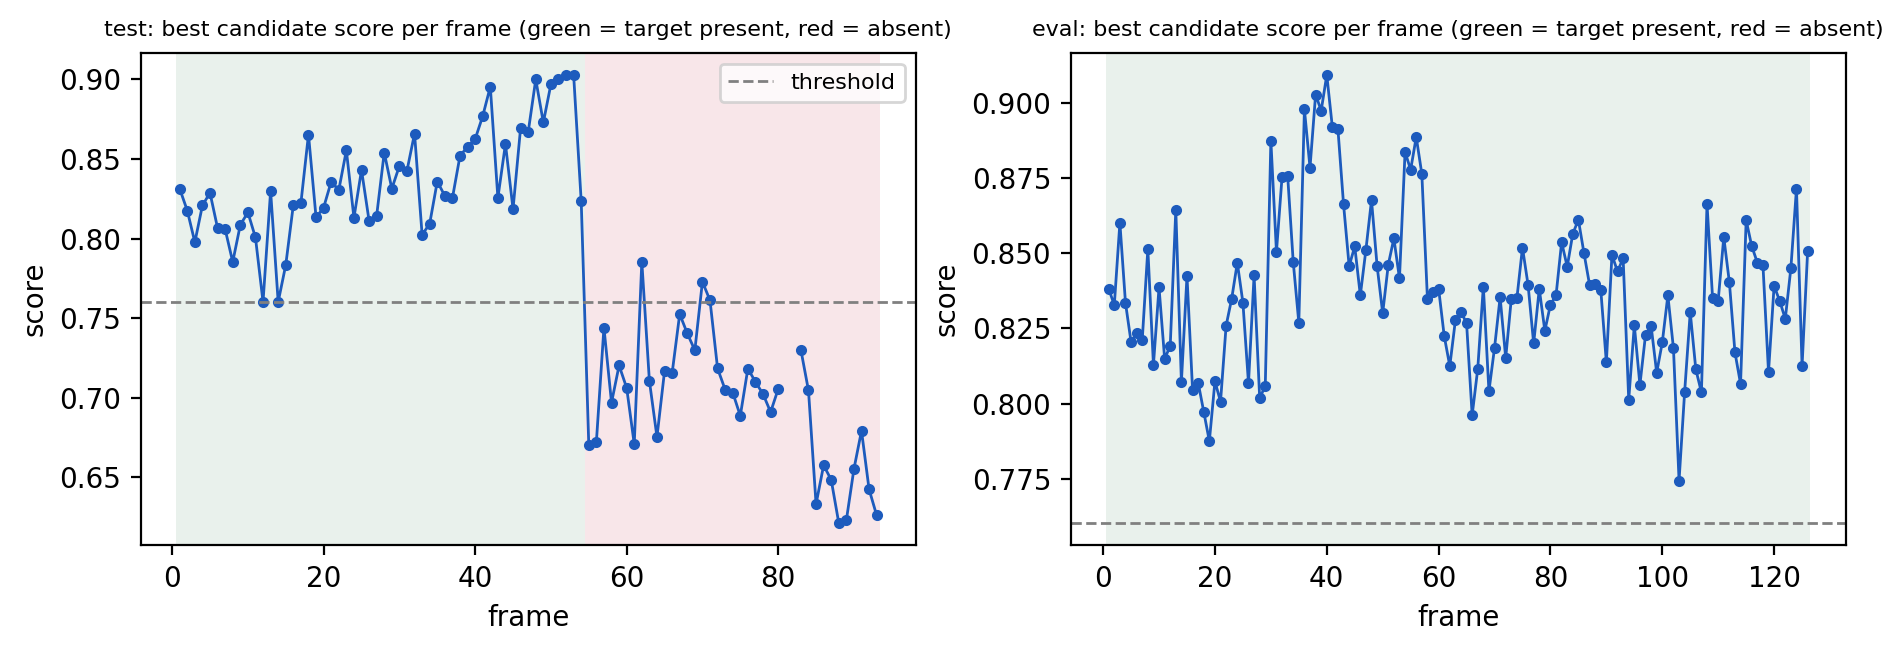
\includegraphics[width=\linewidth]{figures/score_over_time.png}
\caption{Score of the best candidate in each frame, final system. The dashed line is the decision threshold.}\label{fig:time}
\end{figure}

%------------------------------------------------------------------------------------------------
\FloatBarrier
\section{Reflection and limitations}
\textbf{Viewpoint, scale, distance, illumination and occlusion.} The anchors are sharp close-ups, while in the frames the reference boxes are 66--169 px tall (median 126 px) and blurred.
SIFT suffers most: its recall is 0.80 for targets under 80 px tall and 0.69 for larger ones (Table~\ref{tab:size}), and Figure~\ref{fig:sift} shows how few consistent matches survive.
DINOv2 is robust to the change of scale and viewpoint along the camera path: its recall is 0.98--1.00 at both sizes. Multi-resolution anchor views address the resolution mismatch, but no single-resolution ablation isolates their contribution.
Occlusion is permanent in this data: the black hose crosses the red body in every frame and splits the red region in two. The candidate step repairs that by joining the pieces, and no target frame was lost to it. We did not vary the lighting: all recordings are indoors under similar light, so we cannot say how illumination changes would affect the result. The smallest reference box is 66 px tall, so very distant targets were not tested.

\begin{table}[htbp]\centering\small
\begin{tabular}{lrr}
\toprule
System & Target under 80 px tall & Target 80 px or taller \\
\midrule
SIFT & 0.80 (35 frames) & 0.69 (145 frames) \\
DINOv2 & 1.00 (35 frames) & 0.98 (145 frames) \\
DINOv2 + cues (final) & 1.00 (35 frames) & 1.00 (145 frames) \\
\bottomrule
\end{tabular}

\caption{Share of target frames found, by height of the reference box (both sequences pooled, thresholds from \texttt{test}).}\label{tab:size}
\end{table}

\textbf{Do the three anchors contribute equally?} No. Anchor 3 gives the best-matching score most often (115 times, against 96 for anchor 2 and 53 for anchor 1, counted over all real candidates) and has the highest mean similarity. Removing anchor 1 changes nothing, while removing anchor 2 or 3 costs one or two frames on \texttt{eval} (Table~\ref{tab:anchors}).
A single anchor is enough on \texttt{test} but loses recall on \texttt{eval} (anchor 2 alone: 0.94). All three achieve the highest held-out recall, tied with anchors 2 and 3 alone; these recordings show no measurable benefit from adding anchor 1.

\begin{table}[htbp]\centering\small
\begin{tabular}{lrr}
\toprule
Anchors used & \texttt{test} P / R & \texttt{eval} P / R \\
\midrule
all three & 0.95 / 1.00 & 1.00 / 1.00 \\
without anchor 1 & 0.95 / 1.00 & 1.00 / 1.00 \\
without anchor 2 & 0.95 / 1.00 & 0.99 / 0.99 \\
without anchor 3 & 0.98 / 1.00 & 1.00 / 0.98 \\
anchor 1 only & 0.96 / 1.00 & 1.00 / 0.98 \\
anchor 2 only & 0.98 / 1.00 & 1.00 / 0.94 \\
anchor 3 only & 0.92 / 1.00 & 0.99 / 0.99 \\
\bottomrule
\end{tabular}

\caption{Final system with fewer anchors (threshold re-chosen on \texttt{test} each time). P = precision, R = recall.}\label{tab:anchors}
\end{table}

\textbf{Why prints and background score high.} A printed picture of an extinguisher has the same colours, shape and layout as the real one, and both matchers judge appearance only. The histogram even compares colour alone.
SIFT finds the same label-like texture in prints. DINOv2 gives prints a lower but overlapping score (Figure~\ref{fig:scores}).
Depth is the independent evidence that separates them: a print is flat, part of its pillar, and usually smaller than the real object. Depth readings are noisy, so a failed cue lowers the score instead of rejecting the candidate; a hard rejection discarded real extinguishers whose depth was noisy.

\textbf{Effect of candidate generation.} The red-region step found a candidate inside the reference box in every target frame (54 of 54 and 126 of 126), so no target was lost there, and the best candidate overlaps the reference box by at least 70\% in all \texttt{test} frames and 99.2\% of \texttt{eval} frames (the join rule in Section~2.1 is what made the boxes fit).
Candidates and cues already reach 0.95 / 0.96 on \texttt{test} without a matcher (Table~\ref{tab:res_test}). At its selected threshold, that system treats a cue failure as a veto. The final system also uses appearance evidence, which can retain a target despite a failed depth check.
This depends on the target being red and tall; it would not transfer to a differently coloured object. The prints are red too, so they always become candidates and must be removed later.

\textbf{Threshold.} A higher threshold accepts fewer prints but starts to miss real frames; the curves in Figure~\ref{fig:pr} show this trade-off on \texttt{test}.
Without cues, DINOv2 needs a threshold of 0.78 and still has 7 false accepts. With the cue penalty a slightly lower threshold (0.76) gives fewer false accepts and no missed frame. Because \texttt{eval} has no frames without the target, the false-accept side of the threshold can only be checked on \texttt{test}.

\textbf{Accuracy, robustness and processing time.} On the CPU the histogram needs about 4 ms per frame, SIFT 10--17 ms and DINOv2 59--107 ms (Tables~\ref{tab:res_eval} and~\ref{tab:res_test}); these timings exclude depth-feature computation, crop preparation, image reads, threshold decisions and model initialisation. They are partial processing times, including for the no-matcher system. DINOv2 has the highest recall with cues on these recordings, at about six times the cost of SIFT, which is still fast enough for the 4 frames per second of the recordings.

\textbf{Generalisation.} The 219 adjacent frames come from one object and one room. Recognition of a different real extinguisher with similar colour and size, and held-out target-absent decoy rejection, remain untested.

\textbf{Other limitations.} One object and one room were used. The thresholds are tuned on only 93 frames. The cues need a depth frame within 100 ms (median gap 28 ms); depth is unreliable at object edges. We labelled the frames ourselves with a red-region guess as a starting point. The baseline reuses the red candidates and is therefore stronger than a plain global histogram would be.

%------------------------------------------------------------------------------------------------
\FloatBarrier
\section{Contributions}
Each member owns the modules below and presents the matching slides; every member can explain the whole pipeline.

\begin{center}\small
\begin{tabular}{lp{9cm}}
\toprule
Member & Main responsibility \\
\midrule
Achyuth Kumar Baddela & Data loading and depth pairing, candidate regions and the hose-join rule, anchor preparation, the three matchers (histogram, SIFT, DINOv2 with multi-resolution anchor views); slides 1--4. \\
Suresh Balaraman & Labelling tool and the reference labels, evaluation protocol and metric definitions, description of the sequences; slides 5--6. \\
Sathish Kumaresan & Depth cues and their thresholds, decision rule and threshold selection, the seven-system comparison, anchor and size analysis, figures and demo video, README, report and slides 7--11. \\
\bottomrule
\end{tabular}
\end{center}

%------------------------------------------------------------------------------------------------
\section{Reproducing the results}
\begin{verbatim}
pip install -r requirements.txt    # CPU PyTorch: see the first lines of the file
python src/label_tool.py prelabel  # first-guess boxes for the labelling tool
python src/label_tool.py           # label the frames at http://localhost:8000
python src/pipeline.py             # score all candidates (about a minute; the
                                   #   first run downloads the DINOv2 weights)
python src/evaluate.py             # tune on test, report on eval
python src/evaluate.py analysis    # extra measurements for the reflection part
python src/visualize.py            # figures (after evaluate.py)
python src/make_tables.py          # LaTeX tables of this report
python src/make_demos.py          # both H.264 demos; ffmpeg on PATH
\end{verbatim}
The labels are provided in \texttt{data/labels\_test.json} and \texttt{data/labels\_eval.json}, so the labelling step can be skipped.
The DINOv2 source revision is pinned in \texttt{src/pipeline.py}; weights are downloaded from the official repository on first use. Figure generation also synchronises \texttt{report/figures/}. The demo exporter adds five-second title cards with ffmpeg.

\begin{thebibliography}{9}
\bibitem{lowe2004} D.\ G.\ Lowe. Distinctive image features from scale-invariant keypoints. \emph{International Journal of Computer Vision}, 60(2):91--110, 2004.
\bibitem{oquab2023} M.\ Oquab et al. DINOv2: Learning robust visual features without supervision. \emph{arXiv:2304.07193}, 2023.
\bibitem{fischler1981} M.\ A.\ Fischler and R.\ C.\ Bolles. Random sample consensus: a paradigm for model fitting. \emph{Communications of the ACM}, 24(6):381--395, 1981.
\bibitem{bradski2000} G.\ Bradski. The OpenCV library. \emph{Dr.\ Dobb's Journal of Software Tools}, 2000.
\end{thebibliography}

\end{document}
